\documentclass[border=6pt]{standalone}
% Shared preamble for figures.  Each figure is a standalone .tex in
% figures/Unit_X/ that \input's this file; scripts/make-figures.sh turns it
% into images/Unit_X/<name>.svg.  The lesson page and the guided notes both
% use that one SVG, so a figure is drawn once.
%
% Key figures: a figure whose .tex uses \ifkey ... \fi also gets a
% <name>_KEY.svg, built with \keytrue.  Draw the answers inside \ifkey, in
% the key colour (\ans{} for a label, the "answer" style for lines).
\usepackage[T1]{fontenc}
\usepackage{helvet}
\renewcommand{\familydefault}{\sfdefault}
\usepackage{amsmath}
\usepackage{tikz}
\usetikzlibrary{arrows.meta,calc,angles,quotes,decorations.markings,decorations.pathreplacing}
% axis numbers in the text font, not math italic
\pgfkeys{/pgf/number format/.cd,assume math mode=true,1000 sep={}}

\newif\ifkey
\ifdefined\iskey\keytrue\fi
\definecolor{key}{HTML}{C0192B}      % same red as the guided-notes keys
\newcommand{\ans}[1]{\textcolor{key}{\bfseries #1}}

\tikzset{
  % points: \fill (A) circle[radius=\ptr];
  every picture/.append style={line cap=round, line join=round, >={Stealth[length=2.6mm,width=2mm]}},
  fig/.style={thick},
  line/.style={thick,<->},            % a line goes on forever both ways
  ray/.style={thick,->},              % a ray goes on forever one way
  answer/.style={very thick,key},
  % congruence ticks at the middle of a segment: \draw[tick1] (A) -- (B);
  tick1/.style={postaction={decorate},decoration={markings,
    mark=at position .5 with {\draw[thick] (0,-2.2pt) -- (0,2.2pt);}}},
  tick2/.style={postaction={decorate},decoration={markings,
    mark=at position .5 with {\draw[thick] (-1.3pt,-2.2pt) -- (-1.3pt,2.2pt) (1.3pt,-2.2pt) -- (1.3pt,2.2pt);}}},
  tick3/.style={postaction={decorate},decoration={markings,
    mark=at position .5 with {\draw[thick] (-2.4pt,-2.2pt) -- (-2.4pt,2.2pt) (0,-2.2pt) -- (0,2.2pt) (2.4pt,-2.2pt) -- (2.4pt,2.2pt);}}},
  % parallel arrows at the middle of a line: \draw[par1] (A) -- (B);
  par1/.style={postaction={decorate},decoration={markings,
    mark=at position .5 with {\draw[thick] (-2.5pt,-2.5pt) -- (0,0) -- (-2.5pt,2.5pt);}}},
  par2/.style={postaction={decorate},decoration={markings,
    mark=at position .5 with {\draw[thick] (-4pt,-2.5pt) -- (-1.5pt,0) -- (-4pt,2.5pt) (-1pt,-2.5pt) -- (1.5pt,0) -- (-1pt,2.5pt);}}},
  % angle arcs: \pic[ang] {angle = A--B--C};  ang2 for a second matching angle
  ang/.style={draw,thick,angle radius=5mm},
  ang2/.style={draw,thick,angle radius=5mm,double,double distance=1.2pt},
  % right-angle box: \pic[rt] {right angle = A--B--C};
  rt/.style={draw,thick,angle radius=2.6mm},
}
\newcommand{\ptr}{2pt}
% a labelled point: \pt{A}{(x,y)}{above left}
\newcommand{\pt}[3]{\coordinate (#1) at #2; \fill (#1) circle[radius=\ptr] node[#3] {$#1$};}

% coordinate plane with every unit gridded: \cgrid{xmin}{xmax}{ymin}{ymax}{label step}
% Grid lines every unit. Tick labels every <label step> units, but never closer
% than about 0.55cm: on a small grid a step of 1 becomes 2 (or 5), so the
% numbers do not run into each other. Labels sit on white so grid lines
% do not cross them.
% To leave out tick labels where a curve crosses an axis, before \cgrid:
%   \renewcommand{\cgskipx}{5,-5}  \renewcommand{\cgskipy}{5}
\newcommand{\cgskipx}{}\newcommand{\cgskipy}{}
\makeatletter
\newcommand{\cgrid}[5]{%
  \pgfpointxy{1}{0}\pgfmathsetmacro{\cgunit}{\pgf@x}%
  \pgfmathtruncatemacro{\cgs}{max(#5, (\cgunit*#5 < 15.6) ? 2 : #5, (\cgunit*#5 < 7.9) ? 5 : #5)}%
  \draw[gray!45,thin,step=1] (#1,#3) grid (#2,#4);  % step=1 is one unit; the default is 1cm
  % axes run at least 0.5cm past the last grid line, so the arrowheads clear
  % the end tick labels on a small grid
  \pgfmathsetmacro{\cgo}{max(0.4, 14.2/\cgunit)}%
  \draw[thick,<->] (#1-\cgo,0) -- (#2+\cgo,0) node[right] {$x$};
  \draw[thick,<->] (0,#3-\cgo) -- (0,#4+\cgo) node[above] {$y$};
  \pgfmathtruncatemacro{\cgxa}{ceil((#1)/\cgs)*\cgs}\pgfmathtruncatemacro{\cgxb}{\cgxa+\cgs}%
  \pgfmathtruncatemacro{\cgya}{ceil((#3)/\cgs)*\cgs}\pgfmathtruncatemacro{\cgyb}{\cgya+\cgs}%
  \foreach \t in {\cgxa,\cgxb,...,#2} {\edef\cgt{,\t,}\expandafter\in@\expandafter{\cgt}{,\cgskipx,}\ifin@\else\ifnum\t=0\else\node[below,font=\scriptsize,fill=white,inner sep=1pt,yshift=-1pt] at (\t,0) {\t};\fi\fi}
  \foreach \t in {\cgya,\cgyb,...,#4} {\edef\cgt{,\t,}\expandafter\in@\expandafter{\cgt}{,\cgskipy,}\ifin@\else\ifnum\t=0\else\node[left,font=\scriptsize,fill=white,inner sep=1pt,xshift=-1pt] at (0,\t) {\t};\fi\fi}}
\makeatother

\begin{document}
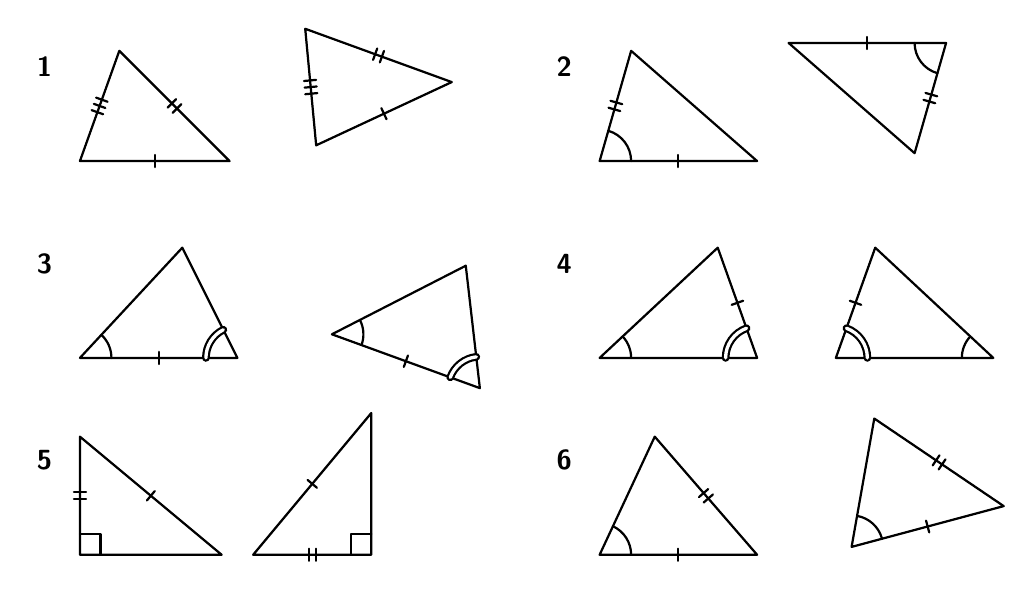
\begin{tikzpicture}[x=1cm,y=1cm]
\coordinate (1x0) at (0,0);
\coordinate (1x1) at (1.9,0);
\coordinate (1x2) at (0.5,1.4);
\draw[fig] (1x0) -- (1x1) -- (1x2) -- cycle;
\draw[tick1] (1x0) -- (1x1);
\draw[tick2] (1x1) -- (1x2);
\draw[tick3] (1x2) -- (1x0);
\coordinate (1y0) at (3,0.2);
\coordinate (1y1) at (4.722,1.003);
\coordinate (1y2) at (2.861,1.68);
\draw[fig] (1y0) -- (1y1) -- (1y2) -- cycle;
\draw[tick1] (1y0) -- (1y1);
\draw[tick2] (1y1) -- (1y2);
\draw[tick3] (1y2) -- (1y0);
\node at (-0.45,1.2) {\textbf{1}};
\coordinate (2x0) at (6.6,0);
\coordinate (2x1) at (8.6,0);
\coordinate (2x2) at (7,1.4);
\draw[fig] (2x0) -- (2x1) -- (2x2) -- cycle;
\draw[tick1] (2x0) -- (2x1);
\draw[tick2] (2x2) -- (2x0);
\pic[draw,thick,angle radius=4.0mm] {angle = 2x1--2x0--2x2};
\coordinate (2y0) at (11,1.5);
\coordinate (2y1) at (9,1.5);
\coordinate (2y2) at (10.6,0.1);
\draw[fig] (2y0) -- (2y1) -- (2y2) -- cycle;
\draw[tick1] (2y0) -- (2y1);
\draw[tick2] (2y2) -- (2y0);
\pic[draw,thick,angle radius=4.0mm] {angle = 2y1--2y0--2y2};
\node at (6.15,1.2) {\textbf{2}};
\coordinate (3x0) at (0,-2.5);
\coordinate (3x1) at (2,-2.5);
\coordinate (3x2) at (1.3,-1.1);
\draw[fig] (3x0) -- (3x1) -- (3x2) -- cycle;
\draw[tick1] (3x0) -- (3x1);
\pic[draw,thick,angle radius=4.0mm] {angle = 3x1--3x0--3x2};
\pic[draw,thick,angle radius=4.0mm,double,double distance=1.2pt] {angle = 3x2--3x1--3x0};
\coordinate (3y0) at (3.2,-2.2);
\coordinate (3y1) at (5.079,-2.884);
\coordinate (3y2) at (4.9,-1.329);
\draw[fig] (3y0) -- (3y1) -- (3y2) -- cycle;
\draw[tick1] (3y0) -- (3y1);
\pic[draw,thick,angle radius=4.0mm] {angle = 3y1--3y0--3y2};
\pic[draw,thick,angle radius=4.0mm,double,double distance=1.2pt] {angle = 3y2--3y1--3y0};
\node at (-0.45,-1.3) {\textbf{3}};
\coordinate (4x0) at (6.6,-2.5);
\coordinate (4x1) at (8.6,-2.5);
\coordinate (4x2) at (8.1,-1.1);
\draw[fig] (4x0) -- (4x1) -- (4x2) -- cycle;
\draw[tick1] (4x1) -- (4x2);
\pic[draw,thick,angle radius=4.0mm] {angle = 4x1--4x0--4x2};
\pic[draw,thick,angle radius=4.0mm,double,double distance=1.2pt] {angle = 4x2--4x1--4x0};
\coordinate (4y0) at (11.6,-2.5);
\coordinate (4y1) at (9.6,-2.5);
\coordinate (4y2) at (10.1,-1.1);
\draw[fig] (4y0) -- (4y1) -- (4y2) -- cycle;
\draw[tick1] (4y1) -- (4y2);
\pic[draw,thick,angle radius=4.0mm] {angle = 4y2--4y0--4y1};
\pic[draw,thick,angle radius=4.0mm,double,double distance=1.2pt] {angle = 4y0--4y1--4y2};
\node at (6.15,-1.3) {\textbf{4}};
\coordinate (5x0) at (0,-5);
\coordinate (5x1) at (1.8,-5);
\coordinate (5x2) at (0,-3.5);
\draw[fig] (5x0) -- (5x1) -- (5x2) -- cycle;
\draw[tick1] (5x1) -- (5x2);
\draw[tick2] (5x0) -- (5x2);
\pic[rt] {right angle = 5x1--5x0--5x2};
\coordinate (5y0) at (3.7,-5);
\coordinate (5y1) at (3.7,-3.2);
\coordinate (5y2) at (2.2,-5);
\draw[fig] (5y0) -- (5y1) -- (5y2) -- cycle;
\draw[tick1] (5y1) -- (5y2);
\draw[tick2] (5y0) -- (5y2);
\pic[rt] {right angle = 5y1--5y0--5y2};
\node at (-0.45,-3.8) {\textbf{5}};
\coordinate (6x0) at (6.6,-5);
\coordinate (6x1) at (8.6,-5);
\coordinate (6x2) at (7.3,-3.5);
\draw[fig] (6x0) -- (6x1) -- (6x2) -- cycle;
\draw[tick1] (6x0) -- (6x1);
\draw[tick2] (6x1) -- (6x2);
\pic[draw,thick,angle radius=4.0mm] {angle = 6x1--6x0--6x2};
\coordinate (6y0) at (9.8,-4.9);
\coordinate (6y1) at (11.732,-4.382);
\coordinate (6y2) at (10.088,-3.27);
\draw[fig] (6y0) -- (6y1) -- (6y2) -- cycle;
\draw[tick1] (6y0) -- (6y1);
\draw[tick2] (6y1) -- (6y2);
\pic[draw,thick,angle radius=4.0mm] {angle = 6y1--6y0--6y2};
\node at (6.15,-3.8) {\textbf{6}};
\end{tikzpicture}
\end{document}
